%www.miktex.org
%\documentclass[a4paper,11pt]{article}
\documentclass[12pt,a4paper,titlepage]{article}%set letterpaper for letter format
%\documentclass[12pt]{report}
%\usepackage{wrapfig}
%\usepackage{shadow}
%\usepackage{epsf}
\usepackage{epsfig}
\usepackage{multicol}
\usepackage{color}
%\usepackage{fancyheadings}
\usepackage{fancyhdr}
\usepackage{fancybox}
%\usepackage{pstricks}
%\usepackage{textpath}
%\usepackage{pst-text}
\usepackage{amsmath}
\usepackage{amssymb}
\usepackage{theorem}
%\usepackage{french}ty

\usepackage[utf8]{inputenc}
\usepackage[french]{babel}
\usepackage[utf8]{inputenc}
\usepackage[french]{babel}
\usepackage[T1]{fontenc}
\usepackage{times}
\usepackage{pifont}
\usepackage{bbding}
\usepackage{wasysym}
\usepackage{manfnt}
\usepackage{hyperref}
\usepackage{glossaries}

% recopie partielle de modele.tex
\setcounter{secnumdepth}{3}
\newfont{\manfnt}{manfnt}

\sloppy
\flushbottom

\parindent 0.8cm
\leftmargini 2em
\leftmarginv .5em
\leftmarginvi .5em
\marginparwidth 20pt
\marginparsep 10pt
\oddsidemargin -0.77cm
\evensidemargin -0.77cm
\topmargin       0mm
\headheight      5mm
\voffset	-14mm
\headsep         4mm
\textheight 24.0cm
\textwidth  18.0cm

%\setcounter{secnumdepth}{3}
%\newfont{\manfnt}{manfnt}
%\setlength{\textwidth}{18.0cm}
%\setlength{\textheight}{24.0cm}
%\setlength{\oddsidemargin}{-0.8cm}
%\setlength{\parindent}{0.8cm}
%\setlength{\headsep}{0.4cm}
%\setlength{\headheight}{-1.25cm}

\newcommand{\ima}[2]{\epsfxsize=#1\epsfbox{#2}}
\makeatletter
\def\@normalsize{\@setsize\normalsize{12pt}\xpt\@xpt
\abovedisplayskip 10pt plus2pt minus5pt\belowdisplayskip \abovedisplayskip
\abovedisplayshortskip \z@ plus3pt\belowdisplayshortskip 6pt plus3pt
minus3pt\let\@listi\@listI}
\def\subsize{\@setsize\subsize{8pt}\xipt\@xipt}
\def\section{\@startsection {section}{1}{\z@}{12pt plus 2pt minus 2pt}
{12pt plus 2pt minus 2pt}{\bf}}
\def\subsection{\@startsection {subsection}{2}{\z@}{12pt plus 2pt minus 2pt}
{12pt plus 2pt minus 2pt}{\bf}}
\makeatother
\def\thesection       {\Roman{section}.}
\def\thesubsection    {\thesection\arabic{subsection}.}
\def\thesubsubsection {\thesubsection\arabic{subsubsection}.}
\newlength{\mylength}
\renewcommand{\baselinestretch}{1.1}
% fin recopie de modele.tex
\pagestyle{plain}

\setlength{\parindent}{0cm}

\title{\textbf{ Mise en place d'un cluster}}
\author{ Bardot Jérôme - Couturier Andy \\ Université de Moncton \\ Département d'informatique \\ Info 4025 }


\makeglossaries

%%%%%%%%%%%%%%%%%%%%%%%%%%%%%
%%%%% DÉBUT DU DOCUMENT %%%%%
%%%%%%%%%%%%%%%%%%%%%%%%%%%%%
\usepackage{graphicx}
\begin{document}

%\thispagestyle{empty}
%\include{page1}
%\newpage

\pagenumbering{roman}


\pagestyle{fancy}
\pagenumbering{arabic}

\fancyhead[l]{\small \emph{INFO4025}}
\fancyhead[c]{\small \emph{-- C --}}
%\fancyhead[r]{\small \emph{Laboratoire n$^{\circ}$ 2}}
\fancyhead[r]{\small \emph{- Présentation détaillée -}}

\fancyfoot[l]{\small \emph{}}
\fancyfoot[c]{\it \mancube \quad \thepage-\pageref{lastpage} \quad \mancube}
\fancyfoot[r]{\small \emph{}}

%%%%%%%%%%%%%%%%%%%%%%%%%%%%%%%%%%%%%%%%%%%%%%

\maketitle 

%\tableofcontents
%\listoffigures
%\listoftables
%\printglossaries




Dans le cadre de notre cours d’architecture avancés d'ordinateurs, nous avons choisi de nous intéresser aux clusters\footnote{Le cluster est un système informatique composé d'unités de calcul (micro-processeurs, cœurs, unités centrales) autonomes qui sont reliées entre elles à l'aide d'un réseau de communication.}. Notre objectif était la remise en état de fonctionnement du cluster du GRETI\footnote{Advanced Internet Technology Research Group}.\\

Dans ce rapport nous allons traiter les concepts mis en œuvre dans une machine de type cluster. Nous verrons un historique des cluster, ainsi que des exemple de cluster reconnus. Nous nous attarderons sur l'architecture et l'organisation physique d'un cluster. Une fois cet aspect maîtrisé nous pourrons nous intéresser a l'aspect logiciel mis en œuvre dans ce type de machine.\\

A l'heure actuelle la recherche scientifique va bon train, avec l’explosion de l’outil informatique il a fallu trouver des solutions à la résolution de calculs complexes. Les machines dédiées au calcul scientifique ont alors fait leur apparition. D'abord d'imposantes machine elle ont vu leurs tailles
réduire avec l'apparition des microprocesseurs dans les années mille neuf cent soixante dix.\\

Pour les machines dédiées au calcul scientifique il existe différents critères de comparaison : 
Tout d'abord la puissance de calcul exprimé en flops\footnote{FLoting-point Operation Per Second (mettre balise acronyme)}. En effet bien souvent les calcul scientifique utilisent des nombres a virgules flottante afin de conserver de la précision ou tout simplement parce que les calculs nécessite ces même nombres.
Formule ?

Le second critère est la disponibilité. Une machine dédiée au calcul ne peut pas se permettre de s’interrompre mettant à mal un calcul nécessitant plusieurs jours voir plusieurs semaines de traitements. Pour cela chaque élément du cluster doit avoir une tolérance au pannes proportionnelle à la criticité de l’élément. 

Un des critères parfois critique est le coût. En effet la réalité économique est souvent au final le facteur déterminant. En effet un cluster peux coûter cher très cher. Tout d'abord il y a le prix du matériel, avec celui viens parfois le coût d'installation. Avec l'utilisation viens le coût d'entretien et de fonctionnement qui comporte le coût en énergie, le coût de remplacement des pièces défectueuses. On peut également signaler que il es possible de choisir des systèmes d'exploitation payant, ainsi que le support pour celui ci. Si le choix se porte sur un système d'exploitation libre il faudra tout de même prévoir un administrateur système pour maintenir le système et faire l'installation.





\section{\large Introduction et Historique }
\subsection{ Introduction rapide aux machines parallèles }

Il existe plusieurs type de parallélisme. Bien qu'il existe de nombreux nouveaux modèle celui qui reste prédominant est le modéle de Michael J. Flynn. Ce modèle classe les architectures en fonction des flux d'instructions et des flux de données.


\subsection{ Comparaison }
\subsection{ Avantages et Inconvénients }


\section{\large Architecture et Organisation physique du cluster }
\subsection{Présentation du cluster, spécifications techniques}
\subsection{ Avantages et inconvénients du clusters.}
\subsection{ Goulots d'étrangement physique.}
\section{\large Aspects Logiciel et Exploitation du parallélisme} 
\subsection{ Choix du système d'exploitation.}

Notre choix s'est tourné vers un système de type GNU$\backslash$Linux. Nous avons choisi la distribution Scientific Linux et ceci pour plusieurs raisons.
Tout d'abord les machines de type GNU$\backslash$Linux sont dotée de nombreux logiciels libre et performants. Il existe pléthore de documentation et bien que n'ayant pas de service de support bon nombre d'utilisateurs apportent leur expertise a travers les documentations officielles ( des distributions, des logiciels libres) ou bien sur IRC\footnote{Internet Relay Chat}. Scientific Linux est une distribution proche de la distribution Red Hat Entreprise Linux une distribution maintenue par une entreprise. Cette proximité lui permet de supporter les paquets\footnote{Un paquet contient un logiciel ainsi que les scripts permettant de correctement déployer et configurer le logiciel} de RedHat ainsi que les patch de leur noyau. \\
Les systèmes de type GNU$\backslash$Linux sont connu pour leur stabilité et leur robustesse ce qui permet d'avoir une machine capable de tourner plusieurs année sans avoir a faire de mise a jour critique. Sans mise a jour critiques, il est possible de garantir la cohérence de comparaison entre résultats d’exécution. \\
Pour des utilisations serveur ou embarqué la possibilité de se passer d'interface graphique est un vrai atout. En effet ce sont les interfaces graphique les plus consommatrice de ressources. Sur une machine dédié au calcul les calculs vont s’exécuter pendant plusieurs jours et sans autre utilisation utilisateur. \\
L'utilisation de logiciel libre est un autre énorme avantage, l'accès aux codes sources permet une compréhension du fonctionnement de chaque logiciel, de ses forces et ses faiblesses en terme d'allocation et de consommation de ressources.
Les systèmes GNU$\backslash$Linux sont dans la grande majorité des cas respectueux des normes ( POSIX par exemple ).
 



\subsection{ Impact du système d'exploitation.}

Le système a un impact important sur la performance et la stabilité du cluster et donc sur les résultat des calculs. 

\subsection{ Choix du logiciel. (MPI)}

La bibliothèque Open MPI est une implémentation open source de la spécification MPI\footnote{Message Passing Interface} dans sa version 3.
La spécification MPI porte sur l’envoi de message entre processeurs permettant la concurrence. L'objectif de la spécification est de standardiser de façon a fournir des interfaces pratique, portable, efficiente et flexible.

Si au début MPI 

\subsection{ Fonctionnement.}
\subsection{ Impact.}
\subsection{ Charge de travail sur le développeur.}
\section{\large Exemple Réel }
\subsection{ Présentation}
\subsection{ Concept}
\subsection{ Implémentation}
\subsection{ Benchmark}
\subsection{ Résultats}
\section{\large Conclusion, tendance actuelle et future.}
\subsection{ maintenance et amélioration}
\subsection{ tendance}
\section{\large Bibliographie.}
\section{\large Lexique et Acronymes}




Chacun des nœuds d'un cluster est capable de fonctionner de façon indépendante du reste des machines.



Architecture :
L'architecture la plus simpliste est un nœud maître connecté à plusieurs nœud esclave.
La connexion est faite a travers un réseau.

A ce réseau peut être ajouté un réseau parallèle permettant la surveillance des différentes parties du cluster en évitant la surcharge du réseau dédié aux calculs.
Pour la majorité il s'agit de calcul scientifique ayant une complexité tel qu'ils ont besoin de plusieurs heures/jours pour arriver a leur termes.
Cette architecture permet une grande souplesse, les nœuds pouvant être ajoutés ou retirés facilement, chacun étant une unité de calcul a pars entière.
Pour peut qu'il y ai redondance des connectiques, des disques et du nœuds maître cela offre une très bonne tolérances aux pannes.

 
Deux classes de Cluster, la classe I :
Les cluster de type 1 sont conçus avec des pièces bon marché, 
nombreuses source de matériel, plus ou moins facilement upgradable. 
Support des drivers Linux.
Basé sur les standards matériels

La Classe II

Basé sur du matériel cher, bien souvent en provenance que d'un seul fournisseur.
Le support par les drivers peux varier.





\subsection{Les Machines Parallèles}

\begin{figure}[htp]
\centering
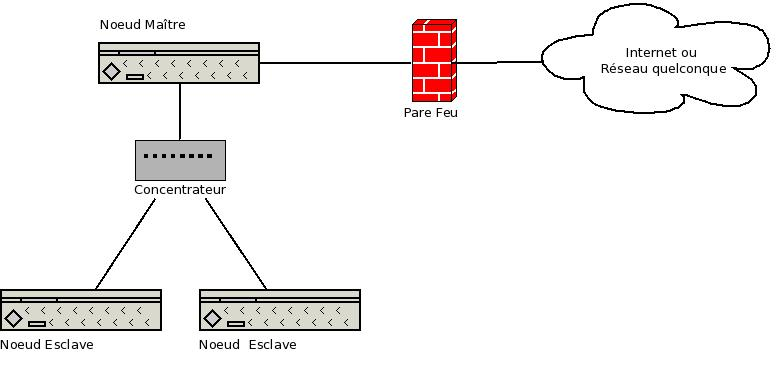
\includegraphics[scale=0.5]{./cluster.jpeg}
\caption{Architecture Type d'un cluster}
\label{}
\end{figure}



un cluster a une mémoire partagé qui communique a travers la mémoire. 
 L'avantage d'utiliser les messages sur une machine SMP, par rapport aux Threads, est que si vous décidez d'utiliser des clusters dans le futur, il est facile d'ajouter des machines ou de scalairiser vos applications.

Avant de passer directement aux opportunités, il y a une distinction très importante qui doit être faite: la différence entre CONCURRENT et PARALLELE. Pour clarifier cette discussion, nous allons définir ces deux termes ainsi:

les parties CONCURRENTES d'un programme sont celles qui peuvent être calculées indépendamment.

Dans un ordinateur parallèle parfait, le rapport communication/calcul devrait être égal et tout ce qui est CONCURRENT pourrait être implémenté en PARALLELE. 

Puisque l'efficacité dépend du rapport communication/calcul, changer juste un composant du rapport ne signifie pas nécessairement qu'une application s'exécutera plus rapidement.


Les parties PARALLELES d'un programme sont celles qui sont exécutées sur des éléments de calculs au même moment.


\newpage

Ressource LinuxHowto 
https://en.wikipedia.org/wiki/FLOPS
http://www.metz.supelec.fr/metz/personnel/vialle/course/Mineure-HPC/notes-de-cours-specifiques/HPC-01-ElementsArchitecturesMachines-2spp.pdf
https://computing.llnl.gov/tutorials/mpi/



L'objectif du projet est de réaliser un \emph{CMS} \footnote{Content Management System} permettant à une communauté d'exister et de communiquer.



-  \href{https://en.wikipedia.org/wiki/FLOPS}{Wikipedia Flops} \\
- \href{http://getbootstrap.com/} \\


people don‚t know about
%alternative \gls{computer} operating systems:
%\glspl{Linux}, BSDs and GNU/Hurd.



%\newglossaryentry{computer}
%{
%name=computer,
%description={is a programmable machine that receives input,
%stores and manipulates data, and provides
%output in a useful format}
%}

%\newglossaryentry{Linux}
%{
%description={is a generic term referring to the family of Unix-like
%computer operating systems that use the Linux kernel}
%}

%\printglossary


\label{lastpage}

\end{document}
